%   % !TEX root = ../../VIII,3_Rahmen-TeX_8-1.tex
%
%
%   Band VIII, 3 N.~??A42
%   Signatur/Tex-Datei: LH_37_05_118
%   RK-Nr. 60334
%   Überschrift: [De flexione laminae elasticae]
%   Modul: Mechanik / Elastizität
%   Datierung: [Ende 1683 (?) bis Mitte 1685 (?)]
%   WZ: (keins)
%   SZ: (keins)
%   Bilddateien (PDF): LH_37_05_118_d1; LH_37_05_118_d2; LH_37_05_118_d3; LH_37_05_118_d4 (insgesamt vier)
%
%
\selectlanguage{ngerman}%
\frenchspacing%
%
\begin{ledgroupsized}[r]{120mm}%
\footnotesize%
\pstart%
\noindent\textbf{Überlieferung:}%
\pend%
\end{ledgroupsized}%
\begin{ledgroupsized}[r]{114mm}%
\footnotesize%
\pstart%
\parindent -6mm%
\makebox[6mm][l]{\textit{L}}%
Aufzeichnung:
LH~XXXVII~5 Bl.~118.
Ein Blatt 4\textsuperscript{o};
Papiererhaltungsmaßnahmen.
Eine Seite auf Bl.~118~r\textsuperscript{o}\!.
Bl.~118~v\textsuperscript{o} ist leer.
\pend%
\end{ledgroupsized}%
%
\vspace*{5mm}%
\begin{ledgroup}%
\footnotesize%
\pstart%
\noindent%
\textbf{Datierungsgründe:}
Die vorliegende Aufzeichnung N.~24 ist inhaltlich mit Untersuchungen über die Spannung der Saiten oder Seile verwandt, die in die erste Hannoveraner Zeit fallen.
Die Ausführung über die Biegung einer elastischen Platte in N.~24 beruht nämlich auf einer Verallgemeinerung der eingangs formulierten Annahme, dass eine Saite gleichmäßig gespannt werde, d.h. in jedem Punkt ihrer Länge der gleichen Spannkraft unterliege.
Auf eine ähnliche Annahme beziehen sich auch weitere Texte in diesem Band \textendash\ etwa N.~7 (S.~\refpassage{LH_35_09_15_001v_gleichSpann_irls-1}{LH_35_09_15_001v_gleichSpann_irls-2}), N.~17 (S.~\refpassage{LH_35_09_15_018r_aequtens-1}{LH_35_09_15_018r_aequtens-2}), N.~20 (S.~\refpassage{LH_35_09_16_008v_gleichSpann_shqe-1}{LH_35_09_16_008v_gleichSpann_shqe-2}) oder N.~26 (S.~\refpassage{LH_38_057r_gleichSpann_kfjg-1}{LH_38_057r_gleichSpann_kfjg-2})~\textendash, die insgesamt auf den Zeitraum vom Sommer 1678 bis Anfang Mai 1685 datierbar sind.
Innerhalb dieser Zeitspanne dürfte wohl auch die Aufzeichnung N.~24 verfasst worden sein.
Ihre Entstehungszeit lässt sich aber insofern weiter einschränken, als Leibniz in der gestrichenen Variante\,\textit{(2a)} zum Textabschnitt \textit{pondus B ... Eodem jure} (S.~\refpassage{LH_37_05_118r_variante_rouv-1}{LH_37_05_118r_variante_rouv-2}) bemerkt, er habe \glqq bereits einmal\grqq\ (\textit{jam olim}) festgestellt, wie viel Spannkraft jedem Punkt einer gespannten Saite zukomme.
Damit könnte er auf die Aufzeichnung N.~6 \textit{De tensione et restitutione} anspielen (S.~\refpassage{LH_35_09_15_001v_gleichSpann_irls-1}{LH_35_09_15_001v_gleichSpann_irls-2}), die sich auf den Zeitraum vom Frühjahr 1679 bis zum Winter 1680/1681 datieren lässt, wobei sich als besonders wahrscheinliches Entstehungsdatum der Winter 1680/1681 erweist (siehe die zugehörigen Datierungsgründe, S.~\pageref{LH_35_09_15_001,022_Datierung}). 
Wenn diese Annahme zutrifft, dann sollte N.~24 nicht vor Ende 1683 verfasst worden sein, da \textit{olim} auf einen geraumen zeitlichen Abstand hindeutet, d.h. wohl mindestens ungefähr drei Jahre.
Zwischen dem Spätsommer 1682 und der ersten Hälfte 1684 befasste sich Leibniz ohnehin besonders intensiv, im Austausch mit E.~Mariotte,\protect\index{Namensregister}{\textso{Mariotte}, Edme, Seigneur de Chazeuil ca. 1620\textendash1684} mit Fragen der Festigkeit und Elastizität (siehe den Textkomplex N.~14 sowie die editorische Vorbemerkung dazu). % S.~\refpassage{}{}
% Vornehmlich die insgesamt zwischen Ende Januar 1683 und der ersten Hälfte 1684 enstandenen Entwürfe N.~??Y\textsubscript{3} und ??Y\textsubscript{7} zeigen thematische Verwandschaft mit der Aufzeihnung N.~??A42.
Und noch in der ersten Hälfte 1685 setzte er sich mit verwandten Themen auseinander, zu denen er durch seine Untersuchung über die Akustik angeregt wurde (siehe den Textkomplex N.~12 sowie die editorische Vorbemerkung dazu).
Somit erweist es sich als plausibel, die Aufzeichnung N.~24 auf den Zeitraum von Ende 1683 bis Mitte 1685 zu datieren.
Eine frühere (nach dem Sommer 1678) oder spätere Entstehungszeit (etwa in den Neunziger Jahren) kann allerdings nicht ausgeschlossen werden. 
\pend%
\end{ledgroup}%
%
\selectlanguage{latin}%
\frenchspacing%
%
%\newpage%
%\vspace{8mm}
%
\newpage
\count\Bfootins=1100
\count\Afootins=1100
\count\Cfootins=1100
%
%\count\Bfootins=1000
%\count\Cfootins=1000
\pstart
\noindent
%
\lbrack118~r\textsuperscript{o}\rbrack\    % % % %    Blatt 118r
%
Sit chorda\protect\index{Sachverzeichnis}{chorda tendibilis}
%
\edtext{tendibilis}{%
\lemma{tendibilis}\Bfootnote{%
\textit{erg.~L}}} 
pondere carens%
\protect\index{Sachverzeichnis}{chorda pondere carens}\protect\index{Sachverzeichnis}{pondus chordae}
%
\edtext{\textit{AB},}{%
\lemma{\textit{AB}}\Bfootnote{%
\textit{erg.~L}}}
%
in summo
%
\edtext{\textit{A}}{%
\lemma{\textit{A}}\Bfootnote{%
\textit{erg.~L}}}
%
adhaerens clavo,\protect\index{Sachverzeichnis}{clavus}
infra vero habens appensum%
\protect\index{Sachverzeichnis}{pondus appensum}
%
\edtext{\edlabel{LH_37_05_118r_variante_rouv-1}pondus \textit{B}.
Hoc posito manifestum est
ubique tensionem\protect\index{Sachverzeichnis}{tensio chordae}
esse aequalem.
Eodem jure\protect\index{Sachverzeichnis}{jus}%
\edlabel{LH_37_05_118r_variante_rouv-2}}{%
{\lemma{pondus}\Bfootnote{\hspace{-0,5mm}%
\textbar~\textit{B} \textit{erg.}~\textbar~%
\textit{(1)}~, a me jam olim
\textit{(2)}~. Hoc posito
\textit{(a)}~a me jam olim definitum est quis in quovis puncto chordae sit casus tensionis\protect\index{Sachverzeichnis}{casus tensionis}
\textit{(b)}~manifestum est \lbrack...\rbrack\ esse aequalem. % ubique tensionem
\textit{(aa)}~Itaque
\textit{(bb)}~Eodem jure%
~\textit{L}}}%
{\lemma{pondus \lbrack...\rbrack\ jure}\Cfootnote{%
In der Variante \textit{(2a)} möglicherweise Anspielung auf N.~6, S.~\refpassage{LH_35_09_15_001v_gleichSpann_irls-1}{LH_35_09_15_001v_gleichSpann_irls-2}.
Der Bezugspunkt könnte aber auch
N.~16, S.~\refpassage{LH_35_09_15_018r_aequtens-1}{LH_35_09_15_018r_aequtens-2} sein.}}}
%
et si lamina Elastica flectatur%
\protect\index{Sachverzeichnis}{lamina elastica}\protect\index{Sachverzeichnis}{flexio laminae}
%
\edtext{vi\protect\index{Sachverzeichnis}{vis incurvans}}{%
\lemma{vi}\Bfootnote{%
\textit{erg.~L}}}
%
aliqua incurvante ad extremum
%
\edtext{\textit{D}}{%
\lemma{\textit{D}}\Bfootnote{%
\textit{erg.~L}}}
%
applicata,\protect\index{Sachverzeichnis}{vis applicata}
ubique aequalis erit tensio,\protect\index{Sachverzeichnis}{tensio laminae}
seu vis aequalis\protect\index{Sachverzeichnis}{vis tendens}
%
\edtext{fiet,
alioqui}{%
\lemma{fiet,}\Bfootnote{%
\textit{(1)}~cum
\textit{(2)}~alioqui%
~\textit{L}}}
%
pars non aeque tensa foret minus fortis,
adeoque tendi se a reliquis fortioribus
quibus obsistit, pateretur,
donec tensio ubique fieret aequalis.\protect\index{Sachverzeichnis}{tensio laminae}
\pend%
%
%
%  \newpage% 
%
\pstart%
Si ponamus in flexione\protect\index{Sachverzeichnis}{flexio laminae}
non augeri longitudinem laminae,\protect\index{Sachverzeichnis}{lamina elastica}
%
\edtext{tantumque fieri vim\protect\index{Sachverzeichnis}{vis tendens}}{%
\lemma{tantumque}\Bfootnote{\hspace{-0,5mm}%
\textbar~ob flexus \textit{gestr.}~%
\textbar\ fieri vim%
~\textit{L}}}
%
in angulis membrilla\protect\index{Sachverzeichnis}{membrillum} connectentibus,
%
tam intus quam extra;
videtur sequi arcum semper esse circularem.\protect\index{Sachverzeichnis}{arcus circularis}
Nam habemus polygonum%
\protect\index{Sachverzeichnis}{polygonum angulorum infinitorum}%
\protect\index{Sachverzeichnis}{polygonum laterum infinitorum}
%
\edtext{aequilaterum aequiangulum
sed angulorum vel laterum infinitorum.}{%
\lemma{aequilaterum}\Bfootnote{%
\textit{(1)}~infinitangulum,\protect\index{Sachverzeichnis}{polygonum infinitangulum}
\textit{(2)}~angulo
\textit{(3)}~aequiangulum sed \lbrack...\rbrack\ laterum infinitorum.%
~\textit{L}}}
\pend%
%
%
\pstart%
Quin etsi ponantur ipsa membrilla extendi et contrahi,
videtur tamen semper \mbox{ubique} aequale debere esse
et membrillorum incrementum,\protect\index{Sachverzeichnis}{membrillum}
et angulorum ratio.
Fortasse si lamina\protect\index{Sachverzeichnis}{lamina elastica} concipiatur ut linea,
sine latitudine et
%
\edtext{crassitie\lbrack,\rbrack%
\protect\index{Sachverzeichnis}{crassities laminae}
omnino exitum\protect\index{Sachverzeichnis}{exitus quaestionis}
non habet quaestio;\protect\index{Sachverzeichnis}{quaestio}}{%
\lemma{crassitie}\Bfootnote{%
\textit{(1)}~res
\textit{(2)}~omnino exitum non habet quaestio;%
~\textit{L}}}
%
quod si jam crassitiem habeat,%
\protect\index{Sachverzeichnis}{crassities laminae}
tunc varius est
%
\edtext{eventus pro crassitiei ratione,
et figura potius solidi\protect\index{Sachverzeichnis}{figura solidi}
nascentis\protect\index{Sachverzeichnis}{solidum nascens}
quam lineae quaerenda,}{%
\lemma{eventus}\Bfootnote{%
\textit{(1)}~pro variis
\textit{(2)}~pro crassitiei ratione,
\textit{(a)}~et pro latitudine in
\textit{(b)}~et figura \lbrack...\rbrack\ lineae quaerenda,% potius solidi nascentis quam
~\textit{L}}}
%
et alia videtur esse superficies solidi%
\protect\index{Sachverzeichnis}{superficies solidi} intus quam
%
\edtext{extra, querendaque}{%
\lemma{extra,}\Bfootnote{%
\textit{(1)}~ut et
\textit{(2)}~quaerendaque%
~\textit{L}}}
%
jam erit linea sectionem solidi%
\protect\index{Sachverzeichnis}{sectio solidi} per
%
\edtext{medium in}{%
\lemma{medium}\Bfootnote{%
\textit{(1)}~supra
\textit{(2)}~in%
~\textit{L}}}
%
concavo pariter et in \makebox[1.0\textwidth][s]{convexo terminans.
Revera tamen
cum crassities sit valde exigua\lbrack,\rbrack\
videtur solidum\protect\index{Sachverzeichnis}{solidum nascens}
pro}
\pend
%
 \vspace{1.5em}%	% Diagramm Fig.~1
  \centerline{\hspace*{-60mm}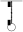
\includegraphics[width=0.14\textwidth]{gesamttex/edit_VIII,3/images/LH_37_05_118_d1.pdf}}%
  \vspace*{0.5em}
  \centerline{\hspace*{-60mm}\lbrack\textit{Fig.~1}\rbrack}%
  \label{LH_37_05_118r_Fig.1}%
%  \vspace{2em}%
%  \newpage%
%
%
%  \newpage% 
  \vspace{-10.0em}%	% Diagramm Fig.~2
  \centerline{\hspace*{60mm}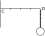
\includegraphics[width=0.268\textwidth]{gesamttex/edit_VIII,3/images/LH_37_05_118_d2.pdf}}%
  \vspace*{0.5em}
  \centerline{\hspace*{60mm}\lbrack\textit{Fig.~2}\rbrack}%
  \label{LH_37_05_118r_Fig.2}%
  %\vspace{1.5em}%
%  \newpage%
%
\newpage
%
%
%  \newpage% 
%	% Diagramm Fig.~3
  \centerline{\hspace*{-60mm}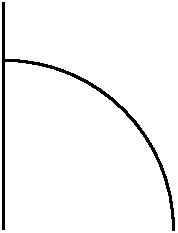
\includegraphics[width=0.18\textwidth]{gesamttex/edit_VIII,3/images/LH_37_05_118_d3.pdf}}%
  \vspace*{0.5em}
  \centerline{\hspace*{-60mm}\lbrack\textit{Fig.~3}\rbrack}%
  \label{LH_37_05_118r_Fig.3}%
%  \vspace{1.5em}%
%  \newpage%
%
%
%  \newpage% 
 \vspace{-11.0em}%	% Diagramm Fig.~4
  \centerline{\hspace*{70mm}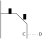
\includegraphics[width=0.25\textwidth]{gesamttex/edit_VIII,3/images/LH_37_05_118_d4.pdf}}%
  \vspace*{0.5em}
  \centerline{\hspace*{65mm}\lbrack\textit{Fig.~4}\rbrack}%
  \label{LH_37_05_118r_Fig.4}%
   \vspace{2.0em}
\pstart
\noindent linea haberi posse;
potest etiam concipi quid prodeat
si crassities\protect\index{Sachverzeichnis}{crassities laminae}
infinite parva\protect\index{Sachverzeichnis}{crassities infinite parva}
intelligatur\lbrack,\rbrack\
quo posito nondum video
quomodo circulum evitare
\edlabel{LH_37_05_118r_saltus_jfdhgv-1}possim.
\edtext{}{%
{\xxref{LH_37_05_118r_saltus_jfdhgv-1}{LH_37_05_118r_saltus_jfdhgv-2}}%
{\lemma{possim.}\Bfootnote{%
\textit{(1)}~Verum
\textit{(2)}~Atque%
~\textit{L}}}}
\pend%
%
%
\pstart%
Atque\edlabel{LH_37_05_118r_saltus_jfdhgv-2}
haec ita prima specie videntur,
sed re melius expensa video
%
\edtext{omnia membrilla}{%
\lemma{omnia}\Bfootnote{%
\textit{(1)}~puncta
\textit{(2)}~membrilla%
~\textit{L}}}
%
sequi directionem imprimentis.\protect\index{Sachverzeichnis}{directio imprimentis}
Ut si in membrillum\protect\index{Sachverzeichnis}{membrillum}
\textit{C} sit impressio\protect\index{Sachverzeichnis}{impressio} \textit{DC},
erit validissima in \textit{C},
obliqua in \textit{B},
nulla in \textit{A}.
\pend
  \count\Bfootins=1200
\count\Afootins=1200
\count\Cfootins=1200
%  \vspace{2em}%
%  \newpage%
%
%
% PR: Ende des Stückes auf Blatt 118r
%
%